%% BioMed\_Central\_Tex\_Template\_v1.06
%%                                      %
%  bmc\_article.tex            ver: 1.06 %
%                                       %

%%IMPORTANT: do not delete the first line of this template
%%It must be present to enable the BMC Submission system to
%%recognise this template!!

%%%%%%%%%%%%%%%%%%%%%%%%%%%%%%%%%%%%%%%%%
%%                                     %%
%%  LaTeX template for BioMed Central  %%
%%     journal article submissions     %%
%%                                     %%
%%          <8 June 2012>              %%
%%                                     %%
%%                                     %%
%%%%%%%%%%%%%%%%%%%%%%%%%%%%%%%%%%%%%%%%%


%%%%%%%%%%%%%%%%%%%%%%%%%%%%%%%%%%%%%%%%%%%%%%%%%%%%%%%%%%%%%%%%%%%%%
%%                                                                 %%
%% For instructions on how to fill out this Tex template           %%
%% document please refer to Readme.html and the instructions for   %%
%% authors page on the biomed central website                      %%
%% http://www.biomedcentral.com/info/authors/                      %%
%%                                                                 %%
%% Please do not use \input{...} to include other tex files.       %%
%% Submit your LaTeX manuscript as one .tex document.              %%
%%                                                                 %%
%% All additional figures and files should be attached             %%
%% separately and not embedded in the \TeX\ document itself.       %%
%%                                                                 %%
%% BioMed Central currently use the MikTex distribution of         %%
%% TeX for Windows) of TeX and LaTeX.  This is available from      %%
%% http://www.miktex.org                                           %%
%%                                                                 %%
%%%%%%%%%%%%%%%%%%%%%%%%%%%%%%%%%%%%%%%%%%%%%%%%%%%%%%%%%%%%%%%%%%%%%

%%% additional documentclass options:
%  [doublespacing]
%  [linenumbers]   - put the line numbers on margins

%%% loading packages, author definitions

\documentclass[twocolumn]{bmcart}% uncomment this for twocolumn layout and comment line below
%\documentclass{bmcart}

%%% Load packages
%\usepackage{amsthm,amsmath}
%\RequirePackage{natbib}
%\RequirePackage{hyperref}
\usepackage[utf8]{inputenc} %unicode support
%\usepackage[applemac]{inputenc} %applemac support if unicode package fails
%\usepackage[latin1]{inputenc} %UNIX support if unicode package fails
\usepackage{graphicx}
\usepackage{amsmath}
\usepackage[switch]{lineno} 
\usepackage{ctable}


%%%%%%%%%%%%%%%%%%%%%%%%%%%%%%%%%%%%%%%%%%%%%%%%%
%%                                             %%
%%  If you wish to display your graphics for   %%
%%  your own use using includegraphic or       %%
%%  includegraphics, then comment out the      %%
%%  following two lines of code.               %%
%%  NB: These line *must* be included when     %%
%%  submitting to BMC.                         %%
%%  All figure files must be submitted as      %%
%%  separate graphics through the BMC          %%
%%  submission process, not included in the    %%
%%  submitted article.                         %%
%%                                             %%
%%%%%%%%%%%%%%%%%%%%%%%%%%%%%%%%%%%%%%%%%%%%%%%%%


% \def\includegraphic{}
% \def\includegraphics{}



%%% Put your definitions there:
\startlocaldefs
\endlocaldefs


%%% Begin ...
\begin{document}

%%% Start of article front matter
\begin{frontmatter}

\begin{fmbox}
\dochead{Research}

%%%%%%%%%%%%%%%%%%%%%%%%%%%%%%%%%%%%%%%%%%%%%%
%%                                          %%
%% Enter the title of your article here     %%
%%                                          %%
%%%%%%%%%%%%%%%%%%%%%%%%%%%%%%%%%%%%%%%%%%%%%%

\title{Population Structure of Radish}

%%%%%%%%%%%%%%%%%%%%%%%%%%%%%%%%%%%%%%%%%%%%%%
%%                                          %%
%% Enter the authors here                   %%
%%                                          %%
%% Specify information, if available,       %%
%% in the form:                             %%
%%   <key>={<id1>,<id2>}                    %%
%%   <key>=                                 %%
%% Comment or delete the keys which are     %%
%% not used. Repeat \author command as much %%
%% as required.                             %%
%%                                          %%
%%%%%%%%%%%%%%%%%%%%%%%%%%%%%%%%%%%%%%%%%%%%%%

\author[
   addressref={aff1},                   % id's of addresses, e.g. {aff1,aff2}
   corref={aff1},                       % id of corresponding address, if any
  % noteref={n1},                        % id's of article notes, if any
   email={charbo24@msu.edu}   % email address
]{\inits{ALC}\fnm{Amanda} \snm{Charbonneau}}

\author[
   addressref={aff3},
   email={kujiratan@gmail.com}
]{\inits{DT}\fnm{David} \snm{Tack}}

\author[
   addressref={aff3},
   email={dworkin@mcmaster.ca}
]{\inits{IMD}\fnm{Ian} \snm{Dworkin}}

\author[
   addressref={aff2},
   email={connerj@msu.edu}
]{\inits{JKC}\fnm{Jeff} \snm{Conner}}

%%%%%%%%%%%%%%%%%%%%%%%%%%%%%%%%%%%%%%%%%%%%%%
%%                                          %%
%% Enter the authors' addresses here        %%
%%                                          %%
%% Repeat \address commands as much as      %%
%% required.                                %%
%%                                          %%
%%%%%%%%%%%%%%%%%%%%%%%%%%%%%%%%%%%%%%%%%%%%%%

\address[id=aff1]{                           % unique id
  \orgname{Department of Genetics, Program in Ecology, Evolutionary Biology and Behavior, Michigan State University}, % university, etc
  %\street{Waterloo Road},                     %
  \postcode{48823}                                % post or zip code
  \city{East Lansing},                              % city
  \cny{USA}                                    % country
}
\address[id=aff2]{
  \orgname{University of Toronto},
  %\street{D\"{u}},
  %\postcode{}
  \city{Toronto},
  \cny{Canada}
}
\address[id=aff3]{
  \orgname{Kellogg Biological Station and Department of Plant Biology, Michigan State University},
  \street{D\"{u}3700 East Gull Lake Drive,},
  \postcode{49060}
  \city{Hickory
Corners},
  \cny{USA}
}

%%%%%%%%%%%%%%%%%%%%%%%%%%%%%%%%%%%%%%%%%%%%%%
%%                                          %%
%% Enter short notes here                   %%
%%                                          %%
%% Short notes will be after addresses      %%
%% on first page.                           %%
%%                                          %%
%%%%%%%%%%%%%%%%%%%%%%%%%%%%%%%%%%%%%%%%%%%%%%

\begin{artnotes}
%\note{Sample of title note}     % note to the article
\note[id=n1]{Equal contributor} % note, connected to author
\end{artnotes}

\end{fmbox}% comment this for two column layout

%%%%%%%%%%%%%%%%%%%%%%%%%%%%%%%%%%%%%%%%%%%%%%
%%                                          %%
%% The Abstract begins here                 %%
%%                                          %%
%% Please refer to the Instructions for     %%
%% authors on http://www.biomedcentral.com  %%
%% and include the section headings         %%
%% accordingly for your article type.       %%
%%                                          %%
%%%%%%%%%%%%%%%%%%%%%%%%%%%%%%%%%%%%%%%%%%%%%%

\begin{abstractbox}
\begin{abstract} % abstract
This paper is about radish and genetics
%\parttitle{First part title} %if any


%\parttitle{Second part title} %if any

\end{abstract}

%%%%%%%%%%%%%%%%%%%%%%%%%%%%%%%%%%%%%%%%%%%%%%
%%                                          %%
%% The keywords begin here                  %%
%%                                          %%
%% Put each keyword in separate \kwd{}.     %%
%%                                          %%
%%%%%%%%%%%%%%%%%%%%%%%%%%%%%%%%%%%%%%%%%%%%%%

\begin{keyword}
\kwd{population structure}
\kwd{weed traits}
\end{keyword}

% MSC classifications codes, if any
%\begin{keyword}[class=AMS]
%\kwd[Primary ]{}
%\kwd{}
%\kwd[; secondary ]{}
%\end{keyword}

\end{abstractbox}
%
%\end{fmbox}% uncomment this for twcolumn layout

\end{frontmatter}

%%%%%%%%%%%%%%%%%%%%%%%%%%%%%%%%%%%%%%%%%%%%%%
%%                                          %%
%% The Main Body begins here                %%
%%                                          %%
%% Please refer to the instructions for     %%
%% authors on:                              %%
%% http://www.biomedcentral.com/info/authors%%
%% and include the section headings         %%
%% accordingly for your article type.       %%
%%                                          %%
%% See the Results and Discussion section   %%
%% for details on how to create sub-sections%%
%%                                          %%
%% use \cite{...} to cite references        %%
%%  \cite{koon} and                         %%
%%  \cite{oreg,khar,zvai,xjon,schn,pond}    %%
%%  \nocite{smith,marg,hunn,advi,koha,mouse}%%
%%                                          %%
%%%%%%%%%%%%%%%%%%%%%%%%%%%%%%%%%%%%%%%%%%%%%%

%%%%%%%%%%%%%%%%%%%%%%%%% start of article main body
% <put your article body there>
\linenumbers
%%%%%%%%%%%%%%%%
%% Background %%
%%
%\section*{Section title}
%\subsection*{Sub-heading for section}
%\subsubsection*{Sub-sub heading for section}
%\paragraph*{Sub-sub-sub heading for section}
%\cite{koon,oreg,khar,zvai,xjon,schn,pond,smith,marg,hunn,advi,koha,mouse}



\section*{Introduction}
Almost seventy percent of the agricultural weeds that plague humans derive from only twelve of the more than 600 plant families{Holm:1978wq}, suggesting that there are only a few evolutionary routes that lead to weediness. Approximately 200 weed species are responsible for more than 90\% of crop losses and these comprise less than one percent of all named plant species{Holm:1978wq, Holm:1997um}. Understanding how these lineages have evolved could guide improvements in weed management {Vigueira:2012ig}.  In addition, agricultural weeds make excellent model systems for understanding rapidly evolving natural populations, as they have recently colonized and adapted to human agricultural fields. 
% * <willpitchers@gmail.com> 2015-11-08T22:00:35.039Z:
%
% > weediness
%
% or at least, that weediness is easy to achieve for some clades than others...?
%
% ^.

That the most devastating agricultural weeds are derived from only a handful of lineages has been known since the mid-seventies {Holm:1977wh}; but despite their staggering costs to the US economy (\$34 billion/year, {Pimentel:2005bw}), research into the evolutionary history of agricultural weeds has been slow to develop. In a recent review, Ellstrand et. al. found that only 13 agricultural weed species were definitively of feral crop origin{Ellstrand:2010ce}. Similarly, Viguera et. al. note that the ancestry of Barnyardgrass (Echinocloa oryzicola), arguably the most costly agricultural weed worldwide, is unknown{Vigueira:2012ig}. This is surprising not only because understanding the evolution of weeds would have many practical benefits, but also because agricultural weeds are an extremely tractable system. 

Research into the evolutionary history of agricultural weeds shares many of the same advantages as studying the crops themselves: recent origin (<10,000 years), economic importance and the availability of historical data{Vigueira:2012ig}, but with the added benefit of having evolved without directed human selection. Agricultural weeds also tend to possess a relatively narrow set of adaptive traits{Baker:1965vt}, many of which will be shared with crop plants{Vigueira:2012ig}. In an agricultural setting, practices like tilling create a narrow window for the weed life cycle, excluding plants requiring more than a few months to go from germination to setting seed. This cyclic and intense disturbance of agricultural fields likely exerts a strong selective force on weeds, selecting for traits such as an annual life cycle, rapid flowering and seed set, and self-pollination or nonspecialist pollinators.
% * <fancy17@gmail.com> 2015-11-02T21:11:51.805Z:
%
% > studying the crops themselves
%
% cite maize Doebley
%
% ^.
% * <fancy17@gmail.com> 2015-11-02T21:11:24.380Z:
%
% >  annual life cycle, rapid flowering and seed set, and self-pollination or unspecialized pollinators
%
% cite barrett? Baker? etc
%
% ^.

Agricultural weeds will often also converge on some traits that are more broadly important for invasive plants, or that share similarities with wild species{Vigueira:2012ig}. For instance, agricultural weeds are often characterized by their ability to colonize disturbed habitats, and such colonization events are often associated with rapid evolution{Reznick:2001gn}, whether the disturbance is natural or caused by human activity{DeWet:1975tv}. 

Although weed evolution is under-researched in general, the evolution of crop mimicry and pesticide resistance in farm systems is relatively well studied and a common feature of agricultural weeds {cite some papers}. Various studies have found evidence for both \textit{de novo} resistance (as reviewed in {Vigueira:2012ig}), as well as rapid selection for traits like acetolactate synthase (ALS) resistance, in response to repeated herbicide use {Tranel:2002uv}. Similarly, it is proposed that vegetative mimicry in weedy sorghum, teosinte, and rices is due to unintentional human selection for seedling traits that closely resemble important crops during hand-weeding {Barrett:1983uu}.  Taken together, these studies suggest that for mimicry and resistance traits to be selected for, the weeds must already be growing in an agricultural field at a rate that causes human intervention, and so are unlikely to be important for initial colonization. Instead, we would expect the strongest initial selection to be on characters that allow survival in agricultural settings. 
% * <willpitchers@gmail.com> 2015-11-08T22:09:35.742Z:
%
% > agricultural settings. 
%
% I like this paragraph -- a very good argument for why I ought top give a f**k.
%
% ^.
% * <willpitchers@gmail.com> 2015-11-08T22:07:11.572Z:
%
% > {cite some papers
%
% Yup, do that! ;-)
%
% ^.
    
One emerging model for studying both rapid evolution and weed evolution is weedy radish, \textit{Raphanus raphanistrum}. Weedy radish has several features that make it an ideal study system to answer questions about both the evolutionary history of agricultural weeds, and which traits rapidly adapt to a field setting. First, it is an agricultural weed of worldwide importance. \textit{Raphanus} is a member of Brassicaceae, one of the twelve major weed families, and it is considered one of the worlds worst weeds {Holm:1997um}. It is the worst dicot weed in Australia {Warwick:2005fm} and a major pest of winter wheat in the southeastern US (ref in grant). Weedy radish primarily infests small grain fields throughout the world {Warwick:2005fm}, and in the last 200 years weedy \textit{R. raphanistrum} has spread to every continent except Antarctica.
% * <willpitchers@gmail.com> 2015-11-08T22:10:56.186Z:
%
% > (ref in grant)
%
% Could JC or ID drop this in!?
%
% ^.

Weedy radish also has several close relatives that can be used for phenotypic and genetic comparison. Crop radishes (\textit{R. sativus}) have been bred to thrive in agricultural environments, and may therefore be predicted to show parallel evolution of some traits. There are also several close wild (non-weedy) relatives which may represent the ancestral states of both the weeds and crops: two named species: \textit{R. pugioniformis} and \textit{R. confusus}; and one or two other subspecies of \textit{R. raphanistrum}. Although there is a great deal of phenotypic diversity in the genus, the species are highly interfertile {Bett:2003eb}, and are known to occasionally hybridize in the wild (cite Ellstrand).

There is also evidence that not all populations of \textit{R. r. raphanistrum} are weeds. A comparative study of weedy \textit{R. r. raphanistrum} from around the world and a single \textit{R. r. raphanistrum} specimen from within its native range (Madrid, Spain) showed that weedy radish flowered in approximately 30 days, after growing only 5 basal leaves. In contrast, the Spanish population took nearly 100 days to flower, had grown more than 25 basal leaves by that time, and a substantial proportion required an over-wintering period (vernalization) to begin flowering. Preliminary investigation of two other populations from the native range, \textit{R. r. landra} and \textit{R. r. maritimus}, showed that they were qualitatively similar to the Spanish population {Sahli:2008kh}. Taken together, these data suggest that a large number of basal leaves and extended time to flowering are ancestral characteristics of the R. r. subspecies, and that weediness is a derived state. This would indicate a major, and rapid, life-history change in the genus, and suggest that early flowering, loss of a rosette, and the switch to an annual lifestyle are likely the first evolutionary steps towards becoming a weed.

However, this previous study was based on genotypic data from only 8 markers, and phenotypic data collected entirely from greenhouse specimens. The dataset was also comprised of a relatively small set of weed populations and a single population from the native range, which may not be representative of native species. To understand the evolutionary history of weedy radish, it is necessary to explore the variation, both within and among populations, of a broader sample of the genus.
% * <willpitchers@gmail.com> 2015-11-08T22:16:57.953Z:
%
% > genus.
%
% this is a neat segue too..
%
% ^.

To meet this goal, we have greatly expanded both the number of genetic markers and the variety of populations, including all named species and subspecies in the genus Raphanus, including 15 populations sampled from the native range, additional weed populations, and 24 crop cultivars from three major groups. To determine population genetic structure, we performed our final SmartPCA and STRUCTURE analysis on 45 radish populations from around the world using 21 SSR and SNP markers. In addition, we grew many of these plants in eight common garden experiments under field conditions to examine genetic differentiation in key phenotypic traits among populations. By increasing the number and diversity of wild species, this study should be more representative of the native variation available for weed evolution, and the defining characteristics of each ecotype. Further, by including a variety of crops, weeds and wild plants, we can look for both genetic and phenotypic similarities among all three ecotypes to plot the evolution of key traits in the genus. We focus on differences in flowering time, which was likely among the first steps in radish weed evolution. 
% * <willpitchers@gmail.com> 2015-11-08T22:19:41.511Z:
%
% > final
%
% ??
%
% ^.

\section*{Methods}

\subsection*{Populations}

To examine genotypic and phenotypic divergence among and between populations, we analyzed \textit{raphanus} seed from 43 populations from around the world, including five of the eight populations of \textit{R. r. raphanistrum} from (2008). In addition, the data set contains 24 commercially available crop varieties, two wild collected populations that are thought to be hybrid or escaped crops, and one population of \textit{Quidproquo confusum} (formerly \textit{Raphanus confusus}), for a total of 69 populations/varieties [Figure:Supp\_Populations].

Of the 70 total populations, a subset of 45 were used in the this analysis [Figure: Populations]. These populations were chosen because we have detailed information about the locations and habitats where each of these samples was collected or purchased. Wild populations were split into two categories: “non-native range \textit{R.r. raphanistrum}” or “native range \textit{R.raphanistrum spp.},” based on country of origin and taxon.

Any population collected from an agricultural field outside the Mediterranean basin was considered to be non-native (6 total). Native range plants were found exclusively in the Mediterranean region, and were collected and assigned to their species and subspecies by experienced taxonomists (15 total). Crop seed was purchased from online retailers with the exception of the three oilseed crops, which were supplied by (a dude from KBS) where they were being grown as a cover crop (24 total).

The remaining populations were either of uncertain genetic origin, were shown to be polyphyletic {ZifferBerger:2014dq}, or were obtained from the Institute for Plant Genetics Crop Plant Research, which does not provide detailed collection notes, only the country of origin for each seed stock. Since we could not determine whether these plants came from agricultural or unexploited land, and our aim was to explore the relationship of weedy (non-native) radish to other radish varieties, these populations were excluded from our analysis. However polymorphism and phenotypic data for these is available in the complete data set on Dryad[website]. Population information for the subset of data used in this study can be found in [Figure: Populations].

\subsection*{Genotyping}

To determine patterns of genetic differentiation among populations of both weedy and native R. raphanistrum and the major groups of crop radish (\textit{R. sativus}) we used a panel of SNP and SSR markers. To create this panel, an initial sequencing of several lines of \textit{R. raphanistrum} was used to assembled and align line-specific contigs against each other. These aligned contigs were then surveyed for line specific SNPS with a custom Python script to allow RFLP markers to be designed around NsiI, PstI, HindIII, EcoRI, BclII, EvoRV, KPNI, and NDEI[Figure: Supp\_Markers]. In addition, the eight SSR markers from Sahli et al. (2008) were also scored on all samples, for a total of 21 markers. Genotyping was completed on 8-10 plants from each of the 54 populations for a total of 543 individuals. However only a subset of 338 individuals from 34 populations were used in the final analyses.

We used two complementary approaches to examine population structure. First we used STRUCTURE {Pritchard:2000uv}using an analysis allowing for admixture with correlated allele frequencies, also called the “F” model, which computes values similar to Fst to model genetic similarities. Our second approach–SmartPCA{Patterson:2006va} –- uses an eigendecomposition optimized for genomic data to reduce the dimensionality of the dataset to orthogonal axes with the most variation. Although this method merely rotates, rather than clusters the data, it can have the effect of revealing structure that was already present, by making it easier to visualize.

\subsection*{STRUCTURE}

We used STRUCTURE {Pritchard:2000uv} version 2.3.4 to cluster individuals by their genetic architecture. Our STRUCTURE analysis was completed using the command line version (v2.3.4), with a burn in of 500,000 cycles followed by one million Markov Chain Monte Carlo (MCMC) iterations. For each potential value of K, we ran 20 separate iterations of the program, each with a different randomization of the data input order. We used the admixture model, which does not require genetic linkage information. As we expected differentiation between populations at neutral markers to be both small and recent, we used the correlated allele frequencies (or F) model, which has more power to detect subtle structure. Our populations were not constrained to a single Fst, and alpha (the degree of admixture) was inferred for the dataset, but not allowed to vary by population, as suggested in the manual. We used the default settings for all priors. We calculated optimal values for K using both the mean log probability of K as in {Pritchard:2000uv} and the largest delta K as described in {EVANNO:2005ga}. The calculations following Evanno were run using the web-based version of Structure Harvester {Earl:2011cn}.

\subsection*{SmartPCA}

We used the ‘SmartPCA’ package (version 9003 from the program Eigensoft 4.2) to analyze our dataset by genetic distance, generating sets of orthogonal vectors analogous to principal components. This method was originally developed for datasets where the number of markers vastly exceeds the number of individuals genotyped, which would be difficult to do a standard PCA on. Our dataset does not fit this expectation, as we have relatively few markers compared to individuals, however we do not expect it to impair the validity of the analysis.

As the SmartPCA algorithms are designed for biallelic markers, each SSR marker was expanded into several biallelic markers as described in {Patterson:2006va} prior to analysis using a custom script. Experimentally determined linkage groups {radishplantbiology:uh} were used as a proxy for chromosomes. Markers that could not be assigned to linkage groups were given unique chromosome numbers. The total number of linkage groups plus singletons was used as the chromosome number (9.)

All SmartPCA and STRUCTURE were run on the HPCC at Michigan State University. We plotted results from SmartPCA and STRUCTURE analysis using custom bash and R scripts {RALanguageandEn:wf}. Scripts for all analyses are available on {https://github.com/ACharbonneau/creepy-barnacle}. SmartPCA results were largely unaffected by inclusion of the \textit{R. confusus} [Figures: SmartPCA and Supp\_SmartPCA]. However, as greatly diverged populations can introduce bias into STRUCTURE analysis, especially using the correlated frequencies model {Kalinowski:2010jr, Falush:2003ts}, \textit{R. confusus} was dropped from the final STRUCTURE analysis.

\subsection*{Phenotyping}

To measure phenotypic variation among populations, we used data from four field and one greenhouse common garden studies (G-03, G-04, F-05, and G-10), performed over a period of several years [Table 1]. These studies all had a relatively large number of individuals per population (mean 48), but a small number of populations per experiment (range 5-9); and while there was some overlap between experiments, each had a unique combination of populations. To validate the results from these trials, we conducted four additional common garden experiments that included many more populations per experiment, but with fewer individuals per population (F-12, F-13, G1-13, and G2-13).

In all experiments, locations of individual plants were randomized with respect to population, and seeds were removed from pods prior to planting to minimize variability in germination times among populations. All plants were monitored daily for germination for the first two weeks, then approximately three times a week thereafter until each had flowered, died, or the pre-determined end of the experiment was reached. We recorded germination date, date of first flower, height of first flower, flower color, and six common floral traits (as per {Conner:1993wn}) on all plants. Additionally, plants in most experiments were scored for total number of rosette leaves from photographs taken on the day they first flowered as well as a variable number of time points throughout the experiment. Watering was as needed.

\subsection*{Modeling}

Phenotypic data from all eight experiments were concatenated for analysis as a single dataset. All models were run using the lme4 package (version 1.1-7) in R (version 3.1.2). Graphs were produced using custom scripts and ColorBrewer (version 1.1-2.) 
To verify the differences in flowering time between native and non-native \textit{R.r. raphanistrum} populations (as presented in {Sahli:2008kh}), and also look for differences between native populations east and west of the Mediterranean Sea, we modeled a subset of the data that only included \textit{R.r. raphanistrum} populations [Figure: Populations]. This model took the form of:

\begin{gather*}
F \sim G + S + D + V + \epsilon\\
% * <fancy17@gmail.com> 2015-11-02T19:49:30.585Z:
%
% > F \sim G + S + D + V + 
%
% Figure out how to give these equation numbers
%
% ^.
\sim X + G x P
\end{gather*}

Where F is the number of whole days from germination to flowering, if available, and the number of whole days from germination until the last day of the experiment, plus one, for plants that survived the duration of the experiment but still hadn’t flowered. G is the geographic region of origin (western or eastern side of Mediterranean, or outside this region). S is a factor representing whether that individuals mother was grown under field or greenhouse conditions. D is the day of year that the plant germinated (1-365) scaled such that 1 is the spring equinox in the northern hemisphere. V is the number of days each plant was vernalized, if any.  The random effect X is the experiment that each plant was in, and accounts for year-to-year variation as well as field vs. greenhouse and other variation in experimental protocols, which are confounded in this study. The random effect GxP accounts for variance among population means within geographic regions.

To look for differences in flowering time among textit{R. raphanistrum} sub-species from within the Mediterranean – whether the \textit{R. raphanistrum} sub-species are more similar to each other, or to other co-localized Raphanus species – we used a subset of the data that included only populations collected from within the Mediterranean region. This model took the form of:

\begin{gather*}
	F \sim U + S + V + \epsilon \\
	\sim X + U x P
\end{gather*}


Where U is a factor representing species or sub-species designation (R.r. raphanistrum, \textit{R.r. landra}, \textit{R.r. maritimus}, \textit{R. pugioniformis} or \textit{R. confusus}), and the other terms are as in the previous model.
To look for differences in flowering time between radish varieties, we used a subset of the data that only included cultivars and used the model:

\begin{gather*}
	F \sim T + \epsilon \\
  \sim X + T x P
\end{gather*}

Where T is a factor representing cultivar variety identity (daikon, European, oilseed or rat-tail), and the other terms are as above.

\section*{Results} 

\subsection*{Clear clustering of species and sub-species, but non-native \textit{R.r. raphanistrum} appears intermediate}

The first two principal components from SmartPCA show clear differentiation between all of the currently accepted species delineations, i.e. \textit{R. raphanistrum, R. sativus,} and \textit{R.r. pugioniformis} [Figure 1: SmartPCA]. In addition to these groupings, we also observe differentiation between some \textit{R. raphanus} sub-species. The distinct grouping of \textit{R.r. landra} and \textit{R.r. maritimus}, in blue, supports the common practice of lumping these two subspecies into \textit{R.r. landra} (e.g.,{Warwick:2005fm}), and separation of these from \textit{R.r. raphanistrum}, in red and gold, is consistent with currently accepted sub-species designations. Although the \textit{R.r. landra} and \textit{R.r. raphanistrum} subspecies form a continuous arc across this genetic subspace, we also find a diffuse boundary within \textit{R.r. raphanistrum} populations, which separates those originating within the Mediterranean from those collected outside the region. Populations taken from inside the Mediterranean region are relatively tightly clustered at either end of the arc (\textit{R.r. landra} in blue, native-range \textit{R.r. raphanistrum} in gold), while populations from outside the region form a more diffuse (red) group in the center of this space. Although non-Mediterranean \textit{R.r. raphanistrum} populations were taken from sites spread across three continents, there is no evidence for isolation by distance among them (data not shown). This is consistent with their likely weedy origin, and being accidentally transported with grain seeds to different locations.(cite seed truck paper)

Exact estimation of K using the STRUCTURE algorithm is difficult, due to our large number of populations/individuals and the relatively small number of markers. Mean log-likelihood suggests K=19 or K=20, while the delta log-likelihood (Evanno) method predicts a K=2 [Figure: Supp\_STRUCTURE]. These two estimates are clearly incompatible with one another; however, major population groupings are robust over this range of Ks, and across multiple runs of the same K. Therefore we used a priori taxonomic groupings consistent with our SmartPCA, varying K between 5, 7 and 9 for the number of groups [Figure 2: STRUCTURE579]. Our results using STRUCTURE are largely consistent with those from SmartPCA, in that native range \textit{R.r. raphanistrum} and \textit{R.r. landra}/maritimus form two clusters, and that the non-native range \textit{R.r. raphanistrum} occupy a middle area between the two. Interestingly, the STRUCTURE results suggest that the non-native range \textit{R.r. raphanistrum} form a genetic gradient between the two native ranges, rather than the somewhat distinct groups suggested by SmartPCA.

Our initial SmartPCA analysis included \textit{Quidproquo confusum} (formerly \textit{Raphanus confusus}) [Figure: Supp\_SmartPCA]. However this species was found to be distant from all the other Raphanus on the first three principal components, consistent with its exclusion from the genus {ZifferBerger:2014dq}, and was therefore excluded from all analyses.

\subsection*{Non-native range \textit{R.r. raphanistrum} show more rapid flowering relative to the native range populations.}

Our first model combines data from many populations of both native and non-native range \textit{R.r. raphanistrum}, as well as several other sub-species, grown under both field and greenhouse conditions. While previous greenhouse studies have shown that non-native range \textit{R.r. raphanistrum} do not require vernalization, and flower more quickly compared to native populations {Sahli:2008kh}, our data is more complex. Consistent with previous observations we observed that the non-native \textit{R.r. raphanistrum} flower significantly more rapidly (p < .001) than the Western range natives, while Eastern native range plants showed an intermediate flowering time (p < 0.05) [Figure 3.] Despite this overall pattern, there remained considerable variation within and between populations [Supp\_PlotRrrPopMeans-1.png], however surprisingly little noise could be attributed to experimental factors like the time of year of germination.
% * <fancy17@gmail.com> 2015-11-02T19:50:06.225Z:
%
% > first model
%
% Refer to model numbers
%
% ^.

\subsection*{Native populations of are phenotypically and genetically weird}

In model two, examining variation between the species and sub-species of the \textit{Raphanus sp.} complex, we found unexpected divergence in flowering times [Figure 4.] Although \textit{R.r. maritimus} and \textit{R.r. landra}, are commonly lumped into a single sub-species {Warwick:2005fm} and cluster genetically at neutral markers [Figure 1], \textit{R.r. landra} populations in our study took about sixty days longer \textit{R.r. maritimus} to flower on average, and had an absolute vernalization requirement [Figure 5]. Further, although \textit{R.r. maritimus}, \textit{R.r. landra} cluster away from native range \textit{R.r. raphanistrum} in both the SmartPCA and STRUCTURE analysis, \textit{R.r. maritimus} is phenotypically intermediate to the other sub-species in both average days to flower, and population frequency of vernalization requirement [Figure 5].

\subsection*{Crop varieties are genetically distinct from both natives and weeds, but show some phenotypic similarity}

All the radish convarieties appeared to cluster together but not with any of the native or non-native radish species and sub-species based on the genetic data. However, while both genetic clustering algorithms separate the crops from all the other populations, results from STRUCTURE [Figure: STRUCTURE579] suggest that the major crop varieties are distinct from each other genetically, while SmartPCA shows that all crop varieties are more closely related to each other than to any of our other radish germplasm. This apparent discrepancy is likely because STRUCTURE uses no measure of genetic distance; groups may thus be separable, but far from equally distant. When the SmartPCA data is plotted to show major crop groups, Daikons form a somewhat distinct subset from the European and other varieties [Figure: Supp\_SmartPCA].

\section*{Discussion}

\textit{Raphanus raphanistrum spp. raphanistrum} is an agricultural weed of small grains with a worldwide distribution, and the genus contains a number of non-weedy congeners and crops. However, the origin and presumed adaptive shift in life-history for the weed is unknown. There are two interconnected questions we wanted to address concerning the origins of weedy radish. First, what are its phylogenetic origins: is it a wild invader, a crop-wild hybrid, an escaped crop or something else; and second how did it acquire weedy traits: was it pre-adapted, or did these traits evolve in situ? We assayed a diverse set of populations of \textit{R.r. raphanistrum}, and its close relatives, to determine how the population structure correlates with two major phenotypes that distinguish weedy radish from non-weedy: days to onset of flowering, and vernalization requirement. 

To determine the phylogenetic origins we constructed a tree using chloroplast sequences. Unfortunately, our phylogenetic analysis could not resolve any relationships below that of the genus, and paralleled the results recently published in {ZifferBerger:2014dq}. From these analyses it is clear that phylogenetic data from more numerous and more variable regions will be necessary to resolve relationships among these closely related taxa. Furthermore, because molecular evolutionary processes including both introgression and incomplete lineage sorting are likely occurring in this recent radiation, it is likely that we will need to analyze sequencing data from multiple individuals of many of these populations in a coalescent framework to resolve a clear species tree (reviewed in Knowles and Kubatko 2010).

Because such a large scale dataset is not yet available, we employed two complementary analyses, STRUCTURE and SmartPCA, to cluster \textit{Raphanus} at presumed neutral markers as an alternative to phylogenetic analysis. There are three commonly accepted possibilities for agricultural weed origins {DeWet:1975tv}, each of which should leave a distinct genetic signature at neutral markers. Weeds could be escaped crops, or wild (native) plants invading a new environment, in which case the weeds should be genetically similar at neutral markers to the crop or native plants respectively. Alternatively, the weeds could be crop-wild hybrids, in which case we would expect the weeds to be somewhat intermediate. In most cases where the origin of agricultural weeds are known, researchers have found them to be escaped crops [refs: sunflower, red rice] or wild-crop hybrids [refs: CA radish, others].

Taken on its own, our SmartPCA results could be interpreted as indicative that the non-native \textit{R.r. raphanistrum} are intermediate between the crops and one (or more) of the native \textit{R. raphanus} sub-species, however the STRUCTURE results do not support this, and the non-native \textit{R.r. raphanistrum} do not appear to share ancestry with the crops at any K from K=3 to K=24. Both STRUCTURE and SmartPCA are unsupervised methods, and both found biologically plausible, and largely congruent, structure; however neither method offers completely unambiguous support for a given hypotheses. Despite this caveat, our results are largely inconsistent with a clear crop-native hybrid or “escaped crop” origins for the weeds.

Instead, both analyses suggest that our agricultural weed samples are genetically intermediate between the native range \textit{R.r. spp. raphanistrum} and \textit{R.r. spp landra/maritimus}, which is consistent with a sub-species hybridization origin for the weeds. This finding is surprising for two reasons. First, these sub-species have over-lapping ranges throughout Spain and France, and are completely inter-fertile [citation], which suggests that hybrids should be widespread. However, local researchers report few or no problems with weedy radish in the region [personal comm.] Second, although the non-native \textit{R.r. raphanistrum} is genetically intermediate, phenotypically it is (uni-directionally) transgressive, with much shorter mean flowering times ( < 20 days) than either of the possible parental \textit{R. raphanistrum} sub-species and no vernalization requirement [Figure: PhenotypeScatter]. Thus, if it did originate as a result of sub-species hybridization, there was likely considerable adaptive evolution in its progenitor for it to become a “true” weed.

The non-native \textit{R.r. raphanistrum} populations are also strikingly similar to each other both phenotypically and genetically; which is especially surprising given the temporal and geographic distribution of our samples. Although this study has only five non-native \textit{R.r. raphanistrum} populations, they were collected as active agricultural weeds from three continents over a span of at least seventeen years; which would suggest that they capture most of the available diversity in weedy radish. However, these populations have a mean pairwise Fst of only .11, barely higher than the mean pairwise Fst of the eleven native \textit{R.r. raphanistrum} (.09), which were all collected in Spain, France and Israel, and were collected over a period of only twelve years. Similarly, in the two axes of greatest differentiation at neutral markers [Figure: SmartPCA] non-native \textit{R.r. raphanistrum} occupies a genetic sub-space nearly identical in extent to that of native \textit{R.r. raphanistrum}. 

Taken together, these data suggest a sub-species hybridization event followed either by recent, long-range dispersal into many sub-populations, or by weed populations interbreeding at relatively high levels despite their geographic distance (as discussed in {Kercher:1996vd}). Our current data cannot conclusively distinguish between these two possibilities. At neutral markers, there is no evident loss of genetic diversity or decrease in heterozygosity among non-native \textit{R.r. raphanistrum} populations as compared to any of the native types, which is a relatively common, if unintuitive feature of invasive species, and may be due to repeated introductions{Blackburn:2015cr}. There is also no appreciable isolation by distance as measured by Fst (data not shown), however, of the fifty-three possible microsatellite alleles, thirteen are found only in single weedy populations, often at high frequency [data not shown – a table for the supplement maybe?]. This may suggest that the weedy meta-population – rather than continuing to interbreed – is more likely to be a group of expanding bottlenecked sub-populations, and sufficient time has not passed for them to diverge as much as far their geographic distance would lead us to expect. 

Interestingly, the clustering patterns suggested for \textit{Raphanus} populations by geographic, genetic, taxonomic and phenotypic data are discordant in a number of instances. For instance, both \textit{R.r. landra} and \textit{R.r. maritimus} are very similar in terms of rosette morphology, are adapted for water-borne seed dispersal {Warwick:2005fm}and are found in the same habitats: primarily in coastal dunes, which would suggest that any flowering time differences should be due to drift. However, \textit{R.r. landra} and \textit{R.r. maritimus} cluster genetically at neutral markers [Figures: SmartPCA and STRUCTURE579], as well as geographically, and in the taxonomic literature {Warwick:2005fm}, which suggests that any phenotypic differences should be due to selection, and that perhaps these are true sub-species. Similarly, native \textit{R.r. raphanistrum} collected from opposite ends of the Mediterranean ocean, with no geographic overlap, are indistinguishable at neutral markers. Why these three sub-species have such phenotypic and genetic incongruities, is unknown, and may be simple drift or indicative of the as-of-yet unresolved phylogenetic relationships of these populations. 

Another situation occurs in the crops (\textit{R. sativus}), which are phenotypically diverse both in our measurements and most cropping traits, but genetically quite closely related [Figure: SmartPCA] at neutral markers. This genetic similarity is at odds with many authors {Yamane:2009ug, Yamagishi:2003jo, Yamane:2005bd, Lu:2008wk, Kong:2010gd, Muminovic:2005uz } who have found considerable diversity among cultivars, and have suggested that there have been multiple origins of crop radish. This difference is likely largely due to sampling. Most of these authors used PCA methods similar to ours, but included only crop cultivars in their analysis, and so have sampled only a fraction of the genetic sub-space of \textit{Raphanus}. Because their data had no (or very few) outgroups, the between group differences are exaggerated. Our SmartPCA analysis actually does show some separation between cultivar types [Figure: Supp\_SmartPCA], these differences are just dwarfed by the variation between crops and the rest of \textit{Raphanus}. Similarly, our own STRUCTURE analysis finds clear divisions between cultivar types using the same data as SmartPCA. However, whereas the graph of SmartPCA clusters maintains some measure of genetic distance, STRUCTURE shows only statistically significant groupings. This means that although the crop groupings in STRUCTURE are equally distinguishable, they are not necessarily equally divergent from each other. Taken together, these data strongly suggest a single origin for \textit{R. sativus}.

The relationship of \textit{R. pugioniformis} to the rest of Raphanus is similarly complex. Originally classified as another sub-species of raphanistrum (then \textit{R.r. rostratus} {Warwick:2005fm}), \textit{R. pugioniformis} {ZifferBerger:2014dq} does not cluster genetically with any of the \textit{raphanistrum} sub-species. In all runs where K is at least 3, STRUCTURE gives \textit{R. pugioniformis} a distinct group, and it falls into an intermediate region between native \textit{R.r. raphanistrum} and the crops [Figure: SmartPCA]. However, it does cluster with native \textit{R.r. raphanistrum} and \textit{R.r. maritimus} in terms of average days to flower and vernalization requirement. Perhaps most strikingly, \textit{R. pugioniformis} is the only wild species to have purple flowers, a trait that otherwise characterizes the crop plants (\textit{R. sativus}). This introduces the possibility that \textit{R. sativus} was originally domesticated from \textit{R. pugioniformis}, although our data cannot distinguish between this scenario and one where \textit{R. pugioniformis} is a crop-native hybrid.

Regardless of questions of phylogenetic origin, it is clear that the evolution of rapid flowering and loss of a vernalization requirement in non-native \textit{R.r. raphanistrum} and the European crops, are both rapid and recent. Although phylogenetic analysis has not yet resolved relationships within the genus, it appears that \textit{Raphanus} is a monophyletic group. That this group is difficult to resolve suggests that observed phenotypic differences have evolved faster than the lineages have split. Similarly, in a series of common garden experiments, non-native \textit{R.r. raphanistrum} takes only 20 days to flower on average, and never requires vernalization, but both the SmartPCA and STRUCTURE analysis find that it is genetically intermediate between two groups with much longer flowering times. This discrepancy between genetic background and phenotype suggests that longer flowering times and a vernalization are the ancestral state, and supports the idea that there has been rapid, recent evolution of these two weed phenotypes. 



%%%%%%%%%%%%%%%%%%%%%%%%%%%%%%%%%%%%%%%%%%%%%%
%%                                          %%
%% Backmatter begins here                   %%
%%                                          %%
%%%%%%%%%%%%%%%%%%%%%%%%%%%%%%%%%%%%%%%%%%%%%%

\begin{backmatter}

\section*{Competing interests}
  The authors declare that they have no competing interests.

\section*{Author's contributions}
    Text for this section \ldots

\section*{Acknowledgements}
  Text for this section \ldots
%%%%%%%%%%%%%%%%%%%%%%%%%%%%%%%%%%%%%%%%%%%%%%%%%%%%%%%%%%%%%
%%                  The Bibliography                       %%
%%                                                         %%
%%  Bmc\_mathpys.bst  will be used to                       %%
%%  create a .BBL file for submission.                     %%
%%  After submission of the .TEX file,                     %%
%%  you will be prompted to submit your .BBL file.         %%
%%                                                         %%
%%                                                         %%
%%  Note that the displayed Bibliography will not          %%
%%  necessarily be rendered by Latex exactly as specified  %%
%%  in the online Instructions for Authors.                %%
%%                                                         %%
%%%%%%%%%%%%%%%%%%%%%%%%%%%%%%%%%%%%%%%%%%%%%%%%%%%%%%%%%%%%%

% if your bibliography is in bibtex format, use those commands:
\bibliographystyle{bmc-mathphys} % Style BST file
\bibliography{bmc\_article}      % Bibliography file (usually '*.bib' )

% or include bibliography directly:
% \begin{thebibliography}
% \bibitem{b1}
% \end{thebibliography}

%%%%%%%%%%%%%%%%%%%%%%%%%%%%%%%%%%%
%%                               %%
%% Figures                       %%
%%                               %%
%% NB: this is for captions and  %%
%% Titles. All graphics must be  %%
%% submitted separately and NOT  %%
%% included in the Tex document  %%
%%                               %%
%%%%%%%%%%%%%%%%%%%%%%%%%%%%%%%%%%%

%%
%% Do not use \listoffigures as most will included as separate files


\onecolumn

\section*{Figures}

% Use this block as a template. W xx %

\begin{figure}[p]
  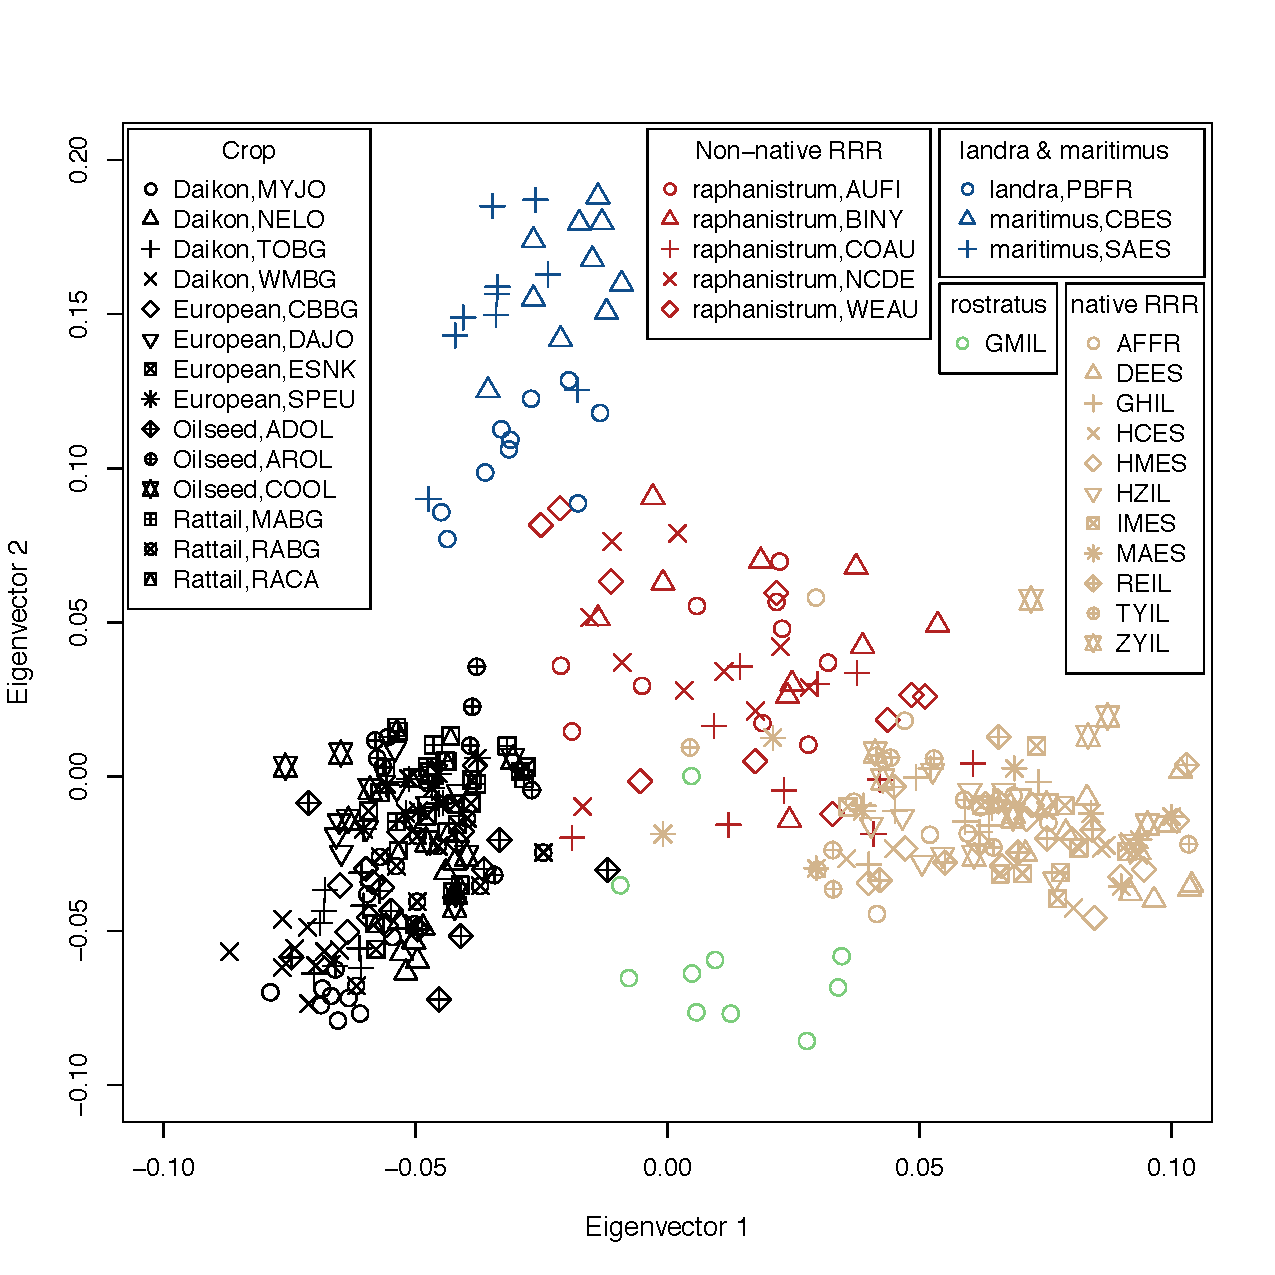
\includegraphics[width=\linewidth]{Figures/SmartPCA.pdf}
  \caption{\csentence{Sample figure title.}
      A short description of the figure content
      should go here.}
      \end{figure}

\begin{figure}[p]
  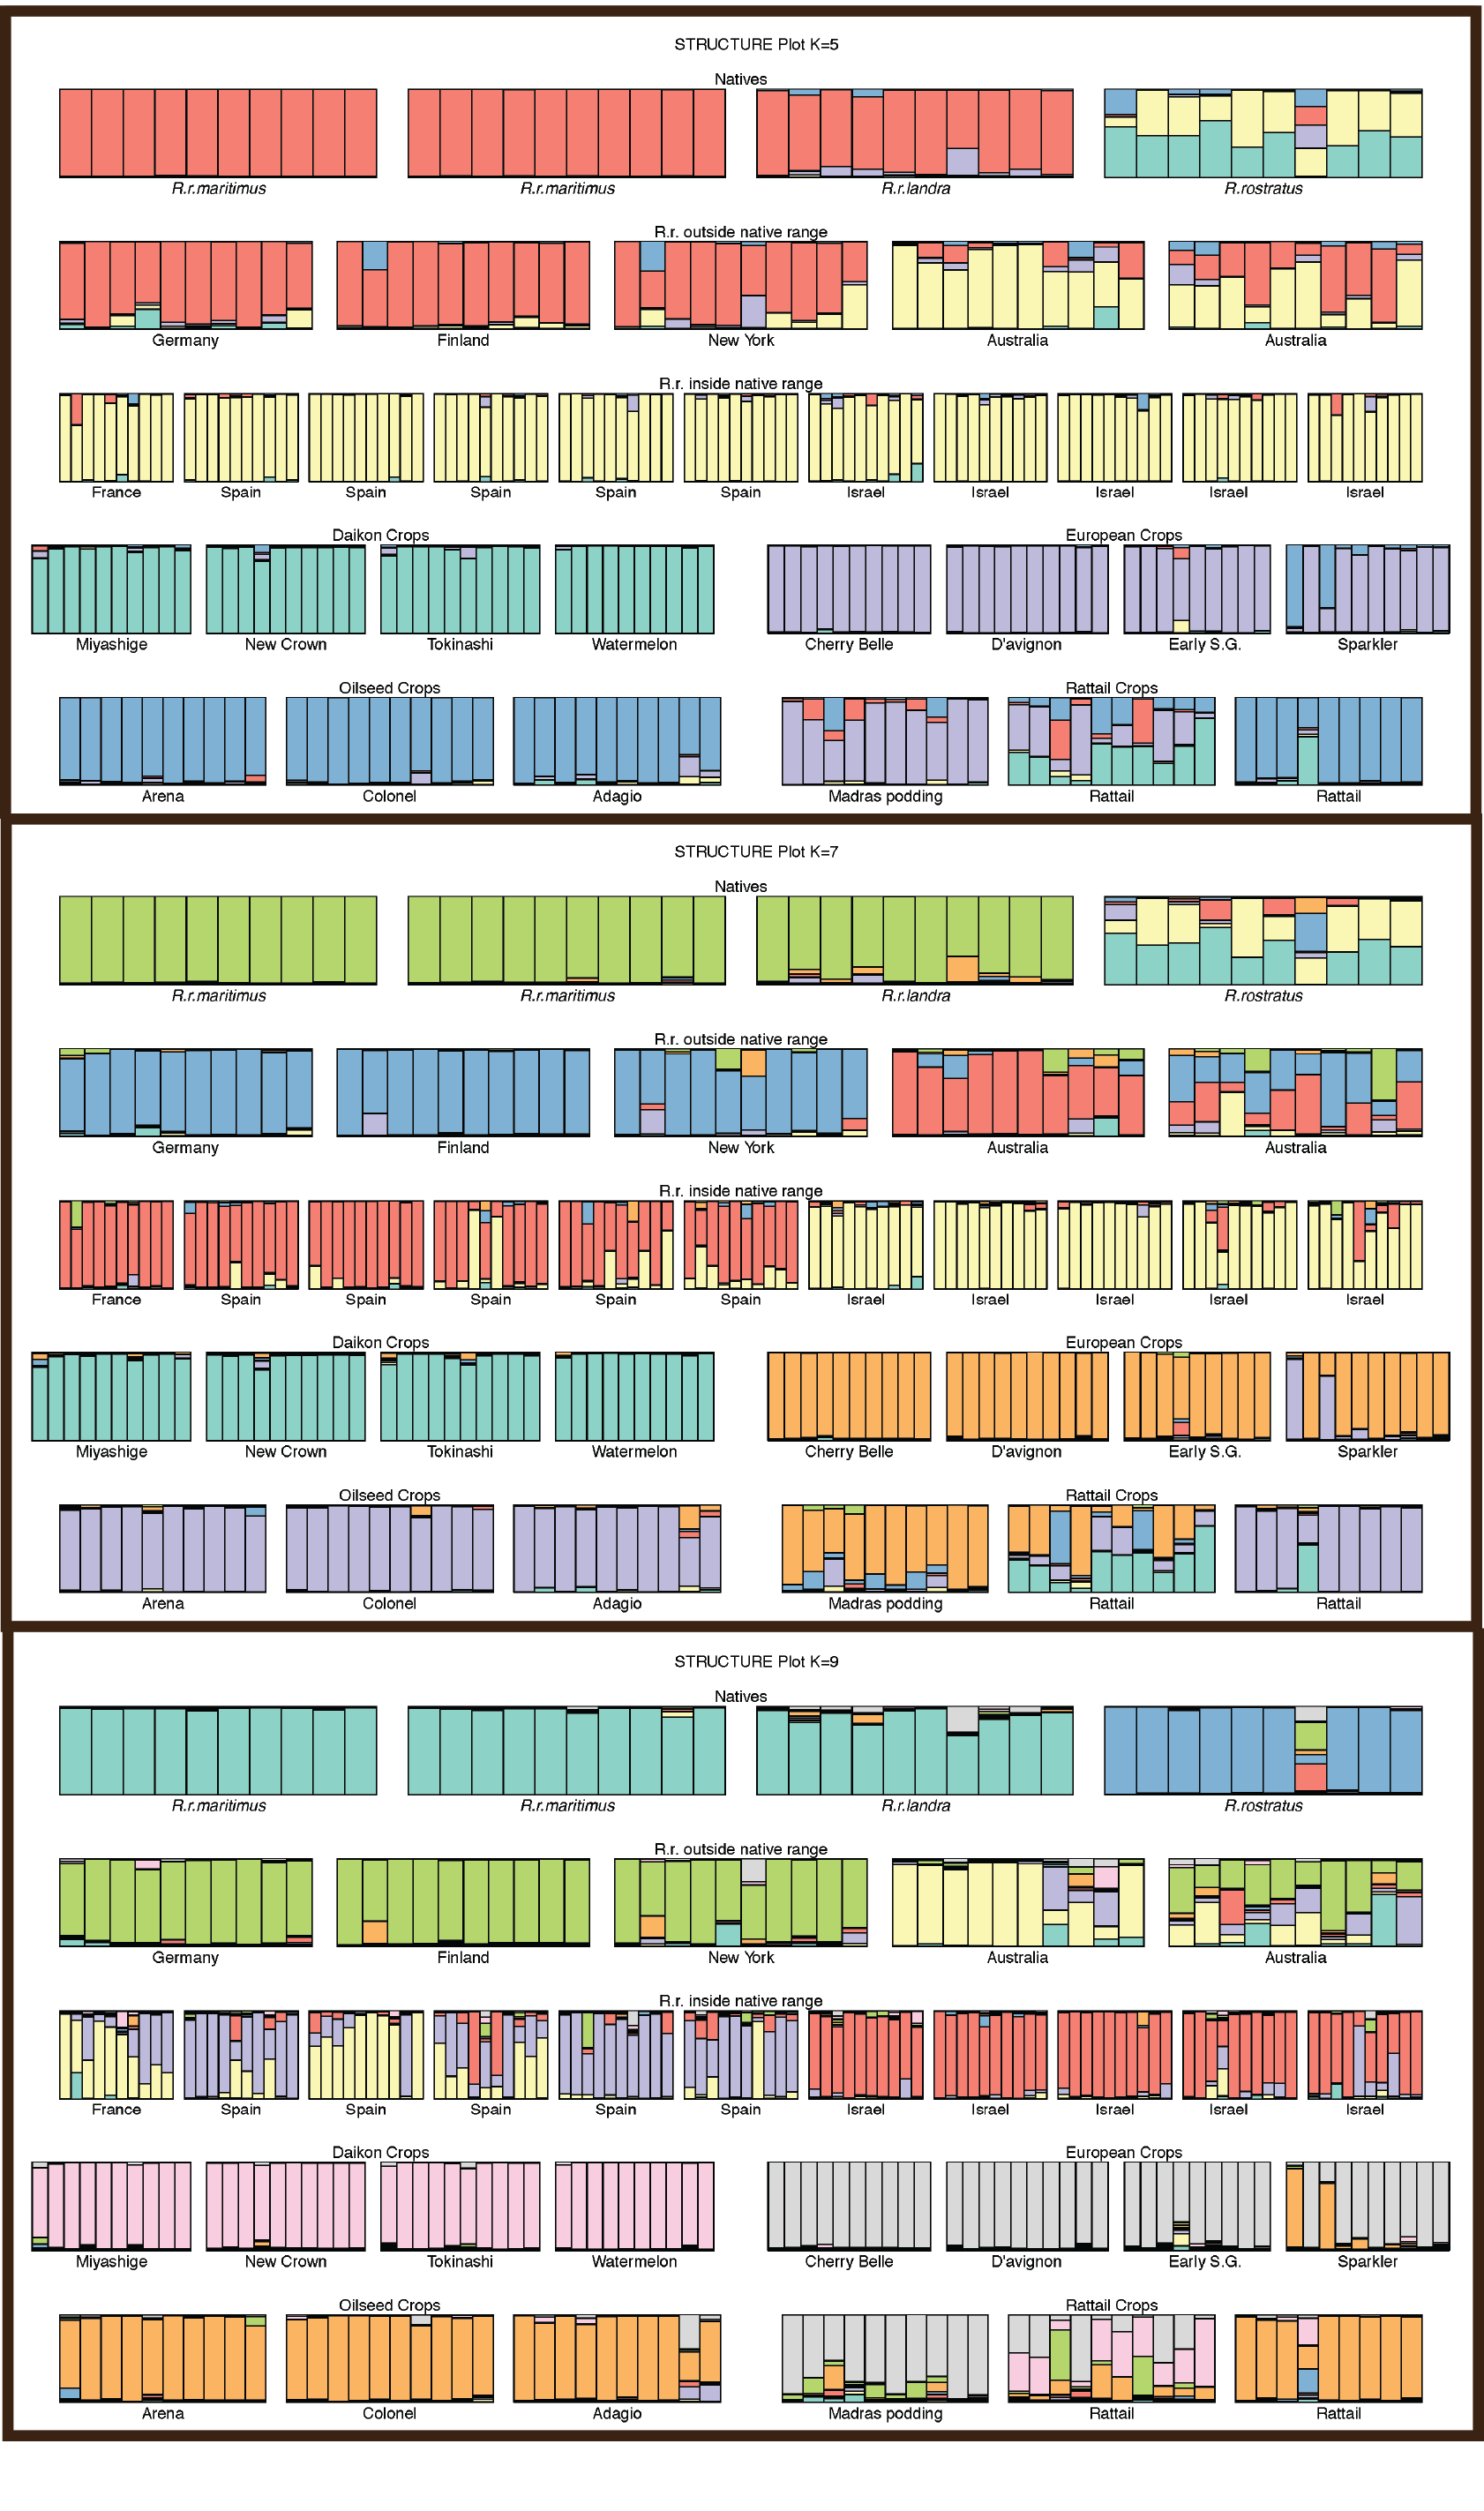
\includegraphics[scale=0.9]{Figures/STRUCTURE579.png}
  \caption{\csentence{Sample figure title.}
      Figure legend text.}
      \end{figure}
      
\begin{figure}[p]
  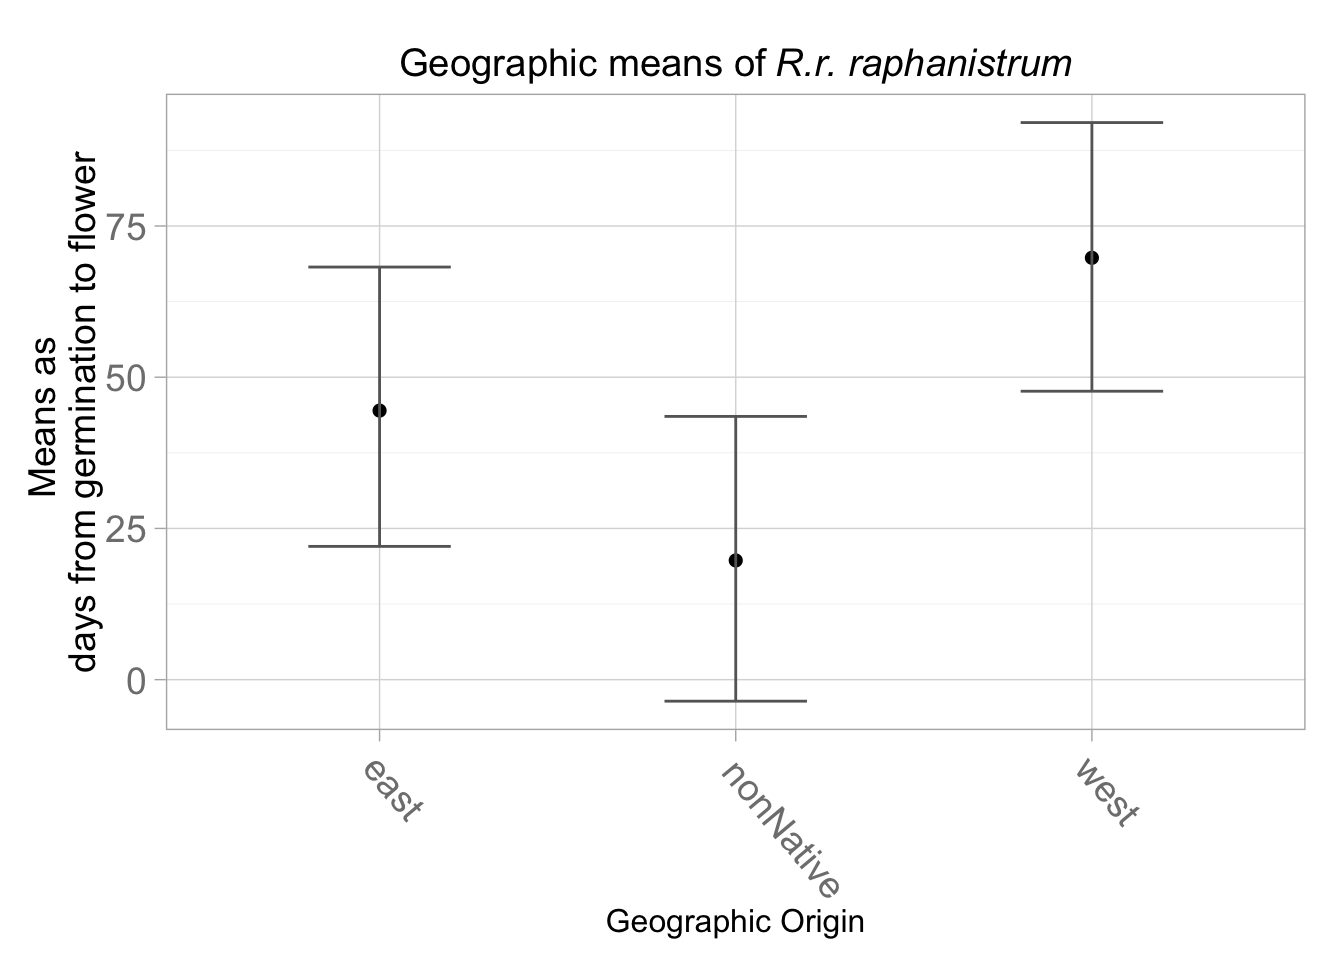
\includegraphics[width=\linewidth]{Figures/PlotRrrMeans-1.png}
  \caption{\csentence{Sample figure title.}
      A short description of the figure content
      should go here.}
      \end{figure}

\begin{figure}[p]
  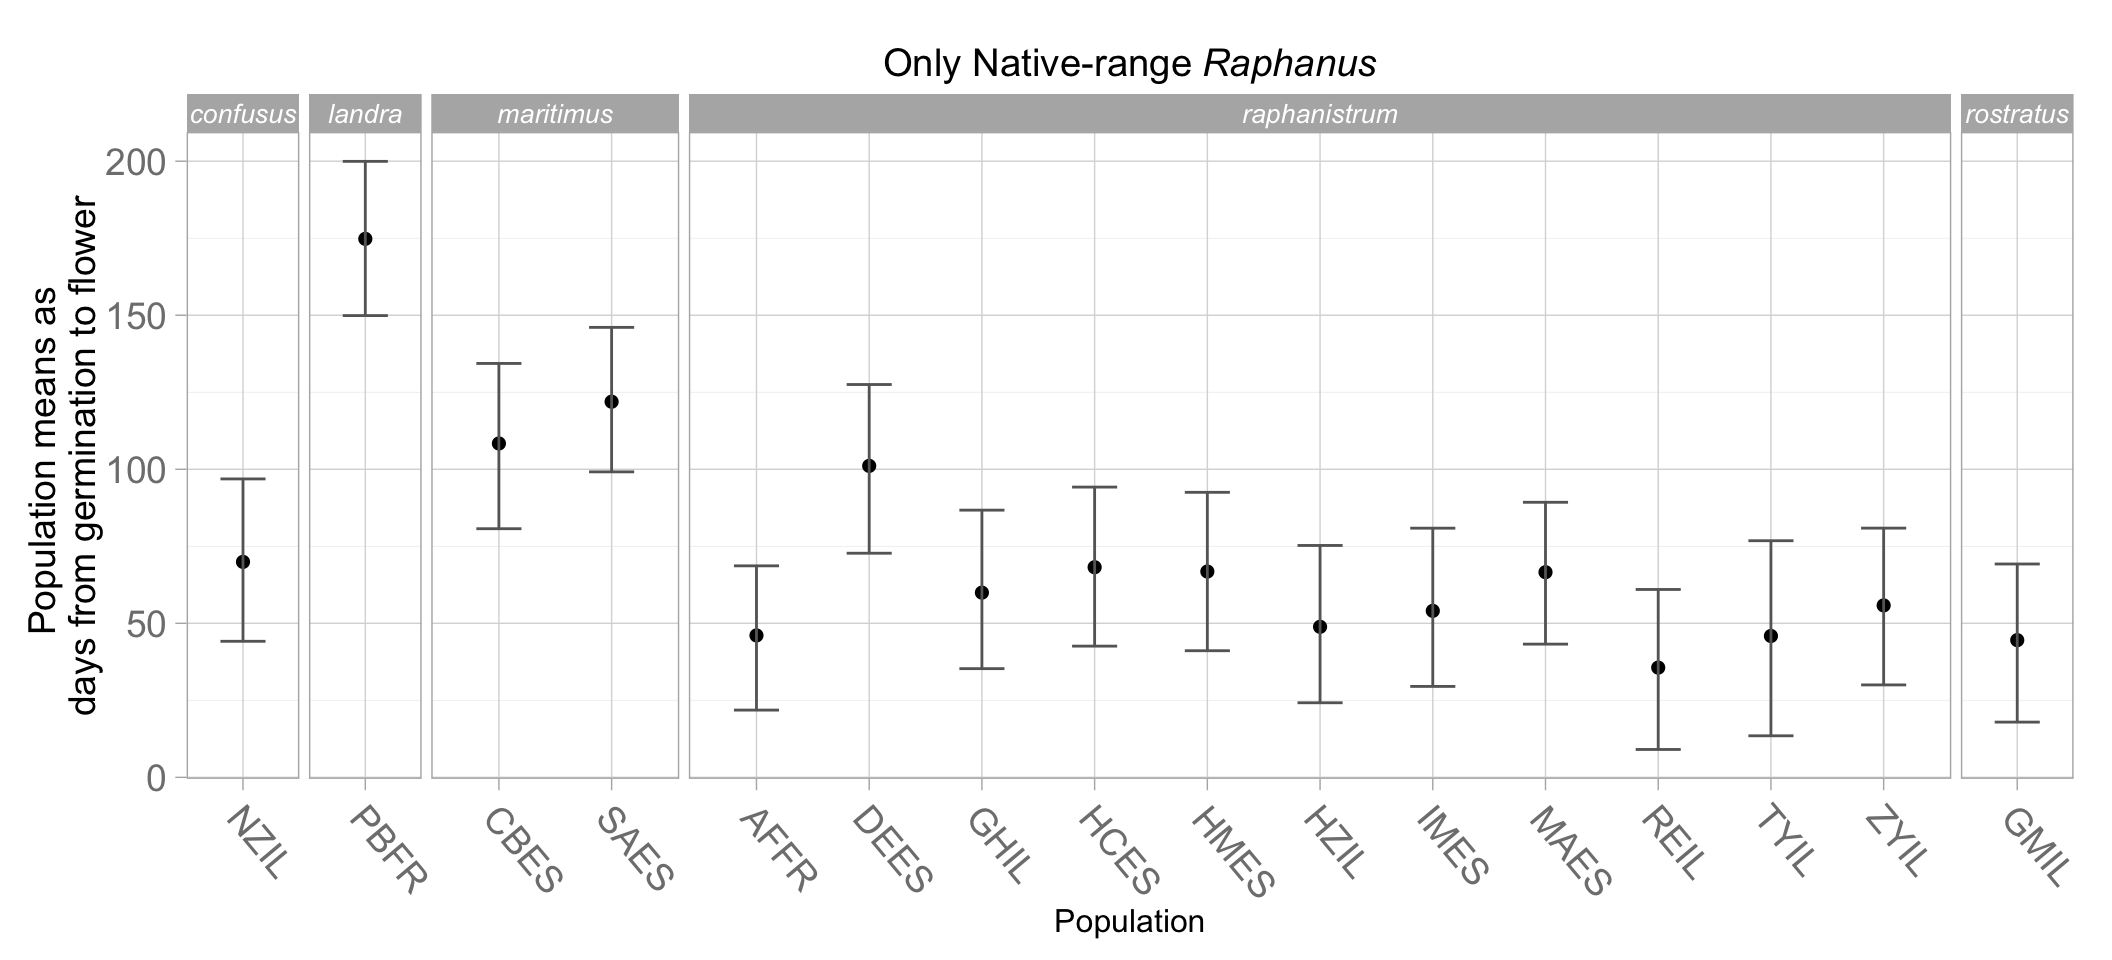
\includegraphics[width=\linewidth]{Figures/PlotNatPopMeans-1.png}
  \caption{\csentence{Sample figure title.}
      A short description of the figure content
      should go here.}
      \end{figure}

\begin{figure}[p]
  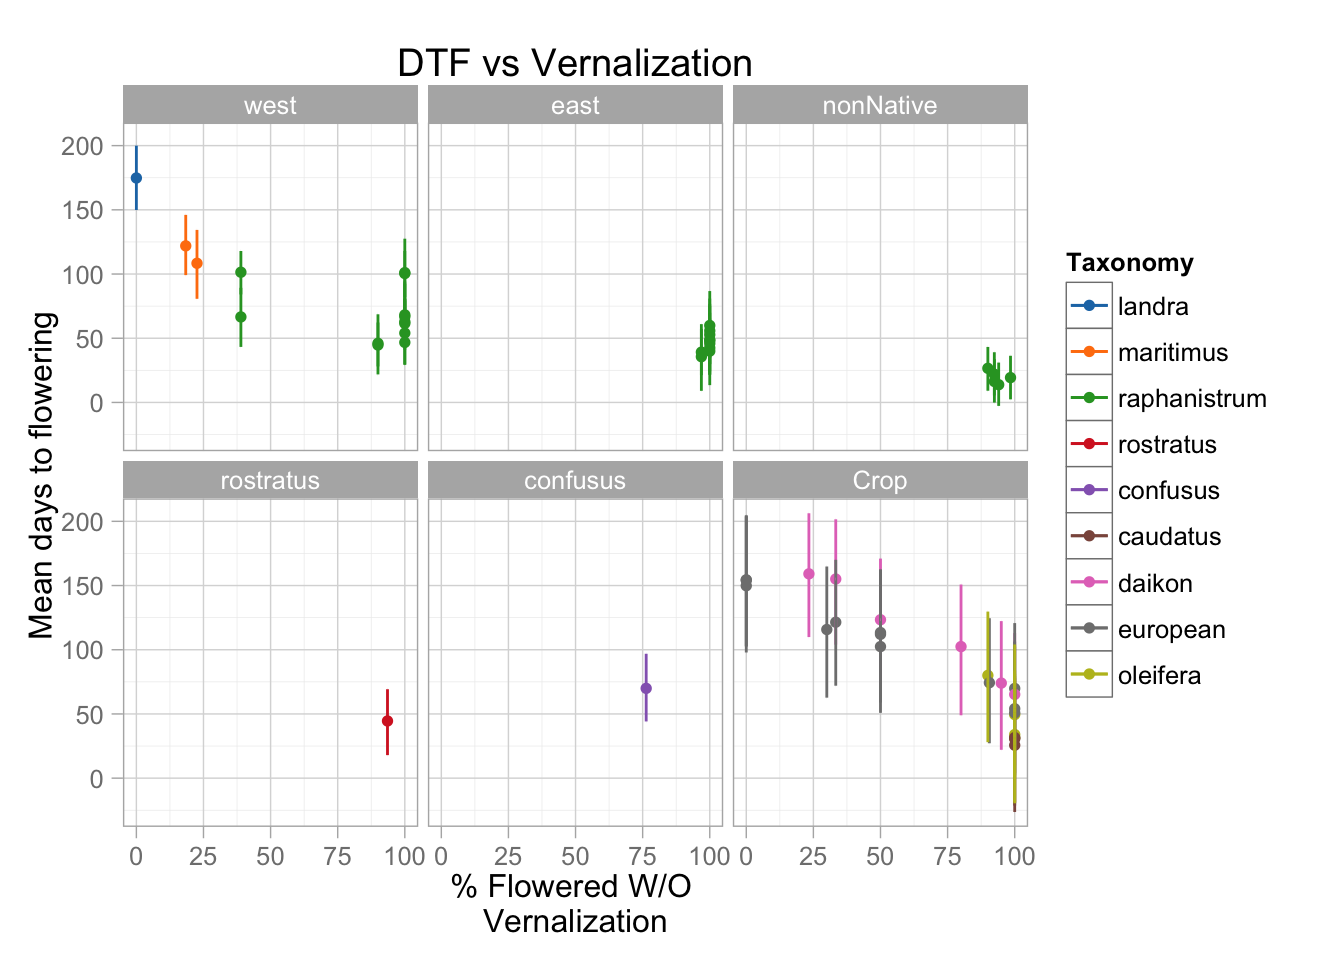
\includegraphics[width=\linewidth]{Figures/PhenotypeScatter-1.png}
  \caption{\csentence{Sample figure title.}
      Figure legend text.}
      \end{figure}


      


%%%%%%%%%%%%%%%%%%%%%%%%%%%%%%%%%%%
%%                               %%
%% Tables                        %%
%%                               %%
%%%%%%%%%%%%%%%%%%%%%%%%%%%%%%%%%%%

%% Use of \listoftables is discouraged.
%%
\section*{Tables}

\begin{table}[p]
\caption{Experiments. This is where the description of the table should go.}
      \begin{tabular}{cccccccc}
        \hline
           Experiment & Year & Location & FieldGH & NPops & NperPop & Description & GermInfo\\ \hline
           G-03 & 2003 & KBS & GH & 9 & 22 - 46 & Sahli parentals & Y\\
           G-04 & 2004 & KBS & GH & 9 & 58 - 142 & Sahli offspring & Y\\
           F-05 & 2005 & KBS & Field & 6 & 64 - 88 & Offspring from Sahli offspring & Y\\
%%           G-06 & 2006 & KBS & GH & 8 & 10 - 31 & random pops & N\\
           G-10 & 2010 & KBS & GH & 5 & 8 - 28 & random pops & Y\\
           F-12 & 2012 & KBS & Field & 18 & 7 - 12 & Many pops, small N & Y\\
           F-13 & 2013 & MSU & Field & 27 & 10 & Many pops, small N & Y\\
           G1-13 & 2013 & KBS & GH & 15 & 10 & Many Crops, small N & Y\\
           G2-13 & 2013 & KBS & GH & 9 & 14 - 30 & Phenotype new pops & Y\\ \hline
      \end{tabular}
\end{table}

\pagebreak


\begin{table}[p]
\caption{Populations. All populations were included in at least one analysis of the paper: Genetic(G) or Phenotypic(P). Variety/Range refers to whether a wild population was collected inside (Native Range) or outside the Mediterranean region; or to the convariety name for cultivated varieties. Source refers to the individual who collected the source populations in the case of wild populations, or the company that cultivar seed was purchased from. Stock/Collection location is the seed company stock number for cultivars, and global position of the source population in the case of wild collected plants.}
      \begin{tabular}{cccccccc}
        \hline
G & P & Population & Variety/Range & Habitat & Source & Stock/Collection location\\ \hline
 \multicolumn{5}{l}{$\boldsymbol{R.r. raphanistrum}$}\\
X & X & AFFR & Native Range & Ag field & Janine Vitou & Fontfroide Abbey, France\\
%% & X & AL & Non-Native Range & Ag field & Lisa Crowfoot & \\
X & X & AUFI & Non-Native Range & Ag field &  & Aura, Finland\\
X & X & BINY & Non-Native Range & Ag field & Jeff Conner & Chenango Bridge, NY\\
%%X & X & COAU & Non-Native Range & Ag field & Lisa Crowfoot & Cowra, Australia\\
X & X & DEES & Native Range & Ag field & Juan Arroyo, et.al & 38º23’25.18”N, 3º29’39.88”W\\
X & X & GHIL & Native Range & Ag field & Barazani et Ziffer-Berger & 32{\ensuremath{^\circ}}10'30.5"N, 34{\ensuremath{^\circ}}56'01.6"E\\
X & X & HCES(A) & Native Range & Ag field & Juan Arroyo, et.al & 37º18'05.93''N, 5º57'57.81''W\\
X & X & HMES(A) & Native Range & Ag field & Juan Arroyo, et.al & 37º16'35.66''N, 5º57'16.80''W\\
X & X & HZIL & Native Range & Ag field & Barazani et Ziffer-Berger & 32{\ensuremath{^\circ}}10'30.5"N, 34{\ensuremath{^\circ}}49'28.9"E\\
X & X & IMES & Native Range & Ag field & Juan Arroyo, et.al & 37º13'16.73''N, 5º58'30.50''W\\
 & X & KAMI & Non-Native Range &  &  & 42{\ensuremath{^\circ}}21'34.6"N, 85{\ensuremath{^\circ}}35'54.2"W\\
%% & X & M3AU & Non-Native Range & Ag field & Lisa Crowfoot & \\
X & X & MAES & Native Range & Undisturbed & César Gómez-Campo & Colmenar Viejo\\
 & X & MAFI & Non-Native Range &  & Kari Lehtila & 60{\ensuremath{^\circ}}33'12''N, 22{\ensuremath{^\circ}}06'53''E\\
%% & X & N3 & Non-Native Range & Ag field & Lisa Crowfoot & \\
%% & X & NAAU & Non-Native Range & Ag field & Lisa Crowfoot & \\
X &  & NCDE & Non-Native Range & Ag field & Caroline Ridley & 52{\ensuremath{^\circ}}58.698'N, 9{\ensuremath{^\circ}}37.865'E; alt: 224\\
%% & X & PG6 & Non-Native Range & Ag field & Lisa Crowfoot & \\
X & X & REIL & Native Range & Ag field & Yuval Sapir & Rehavot, Israel\\
X & X & TYIL & Native Range & Ag field & Yuval Sapir & Tel-Yizhatz, Israel\\
 & X & UKAU & Non-Native Range & Ag field & Lisa Crowfoot & Australia\\
%%X & X & WEAU & Non-Native Range & Ag field & Lisa Crowfoot & Westonia, Australia\\
X & X & ZYIL & Native Range & Ag field & Barazani et Ziffer-Berger & 31{\ensuremath{^\circ}}56'00.4"N, 34{\ensuremath{^\circ}}47'11.4"E\\ \hline
\multicolumn{5}{l}{$\boldsymbol{R.r. landra}$}\\
X & X & PBFR & Native Range & Undisturbed & Janine Vitou & Port Barcares, France\\ \hline
\multicolumn{5}{l}{$\boldsymbol{R.r. maritimus}$}\\
X & X & CBES & Native Range & Undisturbed & César Gómez-Campo & 40 km W. of Santander\\
X & X & SAES & Native Range & Undisturbed & César Gómez-Campo & Noja, Spain\\ \hline
 \multicolumn{5}{l}{$\boldsymbol{R. s. convar. caudatus}$} \\
X & X & MABG & Madras & Crop & Bountiful Gardens & VRA-5060\\
X & X & RABG & Rat's Tail & Crop & Bountiful Gardens & VRA-5070\\
X & X & RACA & Rat's Tail & Crop & John Scheepers & 3870\\ \hline
\multicolumn{5}{l}{$\boldsymbol{R. s. convar. oleifera}$} \\
X & X & ADOL & Adagio oilseed & Crop & MSU & \\
X & X & AROL & Arena oilseed & Crop & MSU & \\
X & X & COOL & Colonel oilseed & Crop & MSU & \\
 & X & OIBG & Oilseed Radish & Crop & Bountiful Gardens & GRA-7378 \\ \hline
\multicolumn{5}{l}{$\boldsymbol{R. s. convar. sativus}$} \\
X & X & CBBG & Cherry Belle & Crop & Bountiful Gardens & VRA-5080\\
 & X & CGBC & Chinese Green Luobo & Crop & Baker Creek Heirloom & Cat\#RD119\\
X & X & DAJO & D'avignon & Crop & John Scheepers & 620.11\\
X & X & ESNK & Early Scarlet Globe & Crop & NK Lawn \& Garden Co & 7576\\
 & X & FGBC & Formosa Giant Luobuo & Crop & Baker Creek Heirloom & Cat\#RD127\\
 & X & FRSI & Flamboyant Long Italian  & Crop & GrowItalian.com & \\
%% & X & GSCA &  & Crop & S. Mazer & 34{\ensuremath{^\circ}}25'13"N, 119{\ensuremath{^\circ}}51'25"W, alt:22 feet\\
 & X & MBBC & Munchener Bier & Crop & Baker's Creek Heirloom & \\
X & X & MYJO & Miyashige & Crop & John Scheepers & 625.11\\
X & X & NELO & New Crown & Crop & John Scheepers & 3860\\
 & X & NTJO & Nero Tondo Black Spanish & Crop & Johnny’s Selected Seeds & \\
 & X & PABS & Patricia & Crop & Burpee's Signature Seeds & \\
 & X & RABS & Raxe & Crop & Burpee's Signature Seeds & \\
X & X & SP[EU/NK] & Sparkler & Crop &	 NK Lawn \& Garden Co & 7583\\
X & X & TOBG & All Seasons Tokinashi & Crop & Bountiful Gardens & VRA-5050\\
X & X & WMBG & Watermelon & Crop & Bountiful Gardens & VRA-5100\\ \hline
\multicolumn{5}{l}{$\boldsymbol{R. s. convar. sativus Niger}$} \\
 & X & LBBC & Long Black Spanish & Crop & Baker Creek Heirloom & \\
 & X & RBBC & Round Black Spanish & Crop & Baker Creek Heirloom & \\ \hline
\multicolumn{5}{l}{$\boldsymbol{R. pugioniformis}$} \\
X & X & GMIL & Native Range & Undisturbed & Yuval Sapir & 32{\ensuremath{^\circ}}30'01.6"N, 35{\ensuremath{^\circ}}24'51.4"E\\ \hline
%%\multicolumn{5}{l}{$\boldsymbol{Hybrid}$} \\
%% & X & BBCA &  &  & Sharon Strauss & 38{\ensuremath{^\circ}}19'02.1"N, 123{\ensuremath{^\circ}}04'15.6"W \\ \hline
 \end{tabular}
\end{table}


%%%%%%%%%%%%%%%%%%%%%%%%%%%%%%%%%%%
%%                               %%
%% Additional Files              %%
%%                               %%
%%%%%%%%%%%%%%%%%%%%%%%%%%%%%%%%%%%

%\section*{Additional Files}
%  \subsection*{Additional file 1 --- Supp\_Markers.xlsx}

\pagebreak
%  \subsection*{Additional file 2 --- Supp\_SmartPCA.png}
 %   Additional file descriptions text (including details of how to
  %  view the file, if it is in a non-standard format or the file extension).  This might
   % refer to a multi-page table or a figure.

  %\subsection*{Additional file 3 --- Supp\_Populations.xlsx}
  %  Additional file descriptions text.
 
% \subsection*{Additional file 4 --- Supp\_STRUCTURE.pdf}
 %   Additional file descriptions text.


\end{backmatter}
\end{document}